% Chapter Template

\chapter{Litterature review}
\label{Chapter1}
%----------------------------------------------------------------------------------------
%	SECTION 1
%----------------------------------------------------------------------------------------
\section{Wood behavior}


Wood is a living material which can be analyzed at different scales. Macroscopic and microscopic scales are, both, really important in order to understand wood behavior.

%-----------------------------------
%	SUBSECTION 1
%-----------------------------------
\subsection{Wood Structure and composition}

In macroscopic scale, wood material is composed of several parts. The first one, the heartwood, is the one with the best mechanical properties. It is considered as the dead part of wood which have a darkest color than the other parts. It is the most used part of the tree for building utilization. That is why, our specimen are made of it. Then, there is the sapwood, a living part of the wood, where the sap circulates. Heartwood is an older sapwood. Around the sapwood, there is the cambium. This part can evolve into sapwood or into the next layer, the bark. All these layers constitute a material which adapts is growth according to the constraints of its environment. That is one explanation of this study choice, which is based on wood analysis.

Microscopic scale show that, heartwood and sapwood are composed of tracheids and vessels linked by parenchymal. They are tubular components of the wood \ref{fig:Fig1}. They are composed of cellulose, lignin, and hemicellulose, which is the link between both type of cells \parencite{Reference1}.
\begin{figure}[th]
	\centering
	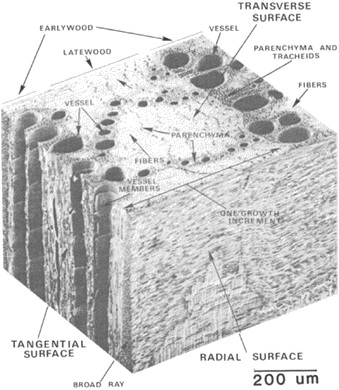
\includegraphics{Figures/Tracheids}
	\decoRule
	\caption[Wood microscopic composition]{Wood microscopic composition, presenting tracheids and vessels}
	\label{fig:Fig1}
\end{figure}
Tracheids allow to transport raw sap (from the ground, to the tree ramification) and elaborated sap (from the ramification to the ground). Some vessels are also perpendicular to wood grain. A phenomenon of capillarity explain how sap can circulate into vessels and tracheids. It is also explained by vegetative transpiration, due to photosynthesis and allow sap movement too \parencite{Reference1}.

Cambium has the role of cellular division \parencite{Reference4} presents it, in his document. Cambium will divide in two different cells. Phloem which is the component of the bark, and xylem which is the cell of sapwood.  All these cells are composed of polymers as cellulose, lignin, and hemicellulose. These cells by their configuration (as the crystal one) are as resistant as steal. Lignin has different interest, like the waterproofing on the cells’ walls. 
Wood is a material which has a specific behavior due to the change of the relative humidity of the middle. This behavior explains that norms forbid its utilization when its internal moisture content exceeds 20\%. Indeed, due to the microscopic properties, it appears that the tracheids expands with moisture content increase. Water present into tracheids and vessels, make it inflated which involve a displacement. On the contrary, when the temperature increase, and relative humidity decrease, tracheids contain less water and retract, but it also involves a displacement. This phenomenon known as Shrinkage - Swelling have an important effect because of the radial and tangential stresses which occurs when all the tracheids expands while the wood is displacement blocked. 
Each wood has a percentage of humidity called saturation fiber point (SFP) which is approximately 30\% amount of water. Under that point, free water contains in tracheids, and vessels will evaporate, and the water contain in cellulose fiber will begin to evaporate too. This effect involve withdrawal. At the opposite, if the amount of water increases and exceed 30\%, there is swelling. 
To provide these effects, wood is often treated and dry before uses. But drying a wood element can produce cracks. When the wood is dry too fast, a located collapse of cells and a crack takes place. The objective in the drying process is to limit the amount of water to nearly 12\%. At its initial state, green wood is considered as a wood full of water. To prevent water effect, and have a 12\% relative humidity inside it, a heating process must be done. Examples can be the stove or a constant ventilation. Indeed, a natural dry will take one year, while an artificial one like, blowing constant hot and humid (at least 70\% of humidity) air, will take one month. 
These information allow to understand the experiments which will be done in this thesis work. But before presenting the experiments, some theoretical knowledges must be reminded. 


%----------------------------------------------------------------------------------------
%	SUBSECTION 2
%----------------------------------------------------------------------------------------

\subsection{An anisotropic and orthotropic material}

Wood is considered as an orthotropic material because the behavior of its mechanical or thermal properties are not the same in its three mutually perpendicular directions. It is a particular anisotropy. This characteristic of the material can be explained by cellular arrangements, growth direction, and other biological elements \parencite{Reference1}. It involves mechanicals difference between each direction.
Wood has good mechanical characteristics. It is resistant in compression thanks to the strength of his structure. It is the same for traction resistance. However, this observation depend on the direction observed.  
The longitudinal direction presented on \ref{fig:Fig2}, is different from the others. Longitudinal direction is the one, which is the less impacted by water effects. Indeed, the tracheids swelling appears on the two others dimensions. So, it is a first independence of this direction on the others. Perpendicular plans, RL and RT are symmetrical. 
Therefore, regarding the tracheid constitution, it is trivial to understand that it is more resistant in terms of traction or compression. Tracheid are composed, \parencite{Reference4} of solid polymers like cellulose or lignin. However, in the others' direction, as tangential or radial one, a tracheid can be separated from the neighbor one, causing a crack due to the separation of tracheids. It is possible when the effort applied on the wood is a perpendicular (perpendicular from the longitudinal direction) traction one. That is why, tests are made on different surface.
\begin{figure}[th]
	\centering
	
\includegraphics{Figures/Wood Surfaces}
	\decoRule
	\caption[Wood surfaces]{Wood surfaces depending on the direction}
	\label{fig:Fig2}
\end{figure}
%----------------------------------------------------------------------------------------
%	SECTION 2
%----------------------------------------------------------------------------------------
\section{Wood species}

Wood are separated into different species and two different groups: the temperate species and tropical species. The literature shows that the tropical species have better resistance due to this more complex microscopic structure characterized by its growth’s environment. This work present experiment on both type of wood. It is important to notice that hardwood (wood from leave trees) and  softwood (wood from needles trees) have different behavior \parencite{Reference2}, but are presented in this work.

%----------------------------------------------------------------------------------------
%	SUBSECTION 1
%----------------------------------------------------------------------------------------

\subsection{Tropical species}

This work will focus on three tropical species, allowing to present woods with different density but from a same area, so dependent to same climatic constraints. Tropical types of woods are located in area, with an equatorial climate or humid tropical climate. Both are characterized by important rains. Equatorial climate has a constant and important pluviometry, while humid tropical climate is composed of a rainy season with torrential rains. Climate is one explanation of the growing differences between tropical and temperate species. In the case of this work, the study will be focused on three tropical species from Congo basin area (central Africa) in Gabon: Okume, Padouck and Iroko. All these species are heartwood ones. 

Okoume specie (Aucoumea klaineana), has the smallest density. It is a wood present in central Africa. The major advantage of this specie is the speed of growth, which is one of the most impressive in wood world. According to CIRAD data \parencite{Reference5}, it has a circumference between 60cm to 120cm and can reach 50m high. The color of this wood is composed of red nuances darkest depending on time. Rupture in compression occurs at a force of nearly 36\si{\mega\pascal} as \parencite{Reference5} present in Okoume wood sheet. It has a density of 0,44 which can be characterized as a light wood. It has a high SFP, equal to 40\% with a tangential withdrawal, superior to the radial one, and is in order of 6,9\%. For all this advantages, it is really used in construction, for carpentry, plywood, or shuttering panels. With a sapwood of approximately, 5\si{\centi\meter}, it allows to work with a large part of the three (heartwood principally). 

Padouck (Pterocarpus soyauxii Taub) is another tropical specie which has a bigger density, about 0,8 \parencite{Reference7}. It is considerate as a heavy wood. This characteristic explains its numerous uses in construction particularly. It can be used for bridge structure, carpentry, naval construction, plywood panels…   From 60\si{\centi\meter} to 100\si{\centi\meter} of diameter it also can reach 50\si{\meter} of high. It is less common and findable than Okoume specie. It must be dry, but it is an interesting wood in terms of natural durability class (heartwood is classed in first durability class)
The Padouck is also a red nuances wood. It is one of the better compression resistance wood in the world, with a resistance until 70\si{\mega\pascal}. It has a SFP around 21\% and a tangential withdrawal of 5\%.

Iroko (Milicia excelsa) is the last wood presented. It is a compromised between the precedent species. It is not a red wood, but a yellow, brown one. It has visible tracheids and a density around 0,65 \parencite{Reference7} . It is also used for many usages, but not particularly construction. It can be used for parquet, woodworking, or cover plywood panels. One of the major advantages of this wood is the transformation of CO2 into calcium oxide crystals. It also considered as a viable wood considering insect and fungus resistance. It has a compression limit equal to 54\si{\mega\pascal} and admit variation of 6\si{\mega\pascal} as mentioned by the CIRAD. It has a tangential withdrawal double from the radial one, this value is 5,4\% and the SFP is 23\%.


%----------------------------------------------------------------------------------------
%	SUBSECTION 2
%----------------------------------------------------------------------------------------

\subsection{Temperate woods}

These trees are located in temperate area and are impacted by temperate climate. It is known that the temperate climate is characterized by four seasons and two important ones, the spring and summer. Indeed, during autumn and winter, trees are not growing waiting for rain and sun, which are essential for its expansion. In spring, the tree needs a lot of water and the cambium produces a large amount of sapwood. This sapwood made in spring is softer and quickly done at the contrary of summer sapwood, heavier with a bigger density. This thesis will compare the three species presented before with a European specie, the Silver Fir. It is a softwood from needles tree. 

The Silver Fir (Abies pectinata). Present on north hemisphere, it is a softwood as Pines or others old trees. As his name undertone, it has a white color, and a circumference between 50 to 80cm. It has a density from 0,45 to 0.60 according to CIRAD data, a SFP about 30\% and a mechanical resistance in compression of 41MPa. The tangential withdrawal is important with a value of 8,7\%, while the radial withdrawal is 4\%. Thanks to it resistance, it is used in carpentry, columns or light frame but must be treated against fungus and insects’ attacks. The main problem with this wood is the water bag contained into the tree. It also has a problem of splitting which prevent uses of some connector in construction field.

%----------------------------------------------------------------------------------------
%	SECTION 3
%----------------------------------------------------------------------------------------
\section{Wood experimentation specimens}


%----------------------------------------------------------------------------------------
%	SUBSECTION 1
%----------------------------------------------------------------------------------------
\subsection{ Double Cantilever Beam (DCB) specimen}

%According to the different article on this test, it appears that it is used mainly with WS and DCB sample. As \parencite{Reference11} presents, it is a method permitting to study the crack tip and then estimate crack length during the wedge split test procedure. Most of the time, it is used in addition of DIC methods. For those reasons, this test is one of the most interesting in the presented case of a mode I study. It uses the compliance method for crack length estimation. 
%The test is simple, as it is visible on \ref{fig:Fig6} it consists of using two arms surrounding the specimen which is fixed to the press by metallic grips. The tested specimen must be adapted to the system, such as ARCAN one, proposed by \parencite{Reference6}. The efforts are applied by an electromechanical press, in this work, the MTS allow to obtain the force applied for a given displacement per second. The chosen grips are simpler than ARCAN ones and allow only mode one tests.
%\begin{figure}[th]
%	\centering
%	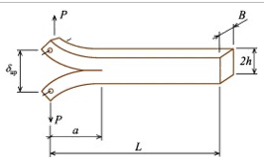
\includegraphics{Figures/DCB Test}
%	\decoRule
%	\caption[DCB Test]{Sheme of DCB Test in mode I, showing the different variables as $\delta_{ap}$, the opening length of the crack lips, a, the crack length, P the applied force and geometrical values of the specimen}
%	\label{fig:Fig6}
%\end{figure}
%A sensor detects the movements of the application point of the forces.
%Therefore, a camera is placed in the axis of the crack in order to use the images and study the crack.

DCB specimens are mainly used in opening mode. The geometry is simple, often rectangular, it has one dimension longer than the two other. The crack propagate in this more important dimension, allowing a displacement of the fracture process zone as presented in \ref{fig:DCB}.
\begin{figure}[h]
	\centering
	
\includegraphics{Figures/DCB}
	\decoRule
	\caption[DCB specimen]{DCB specimen tested by application of a load P}
	\label{fig:DCB}
\end{figure}
The tests on these samples allow the determination of the energy release rate in mode I, which is the parameter that we want to compare. The DCB test specimens permits also to obtain the stress intensity factor.
These specimens are interesting thanks to this important range of propagation of the crack. The compliance method is used on these specimens because of the CTOD, which is easily calculated. Indeed, it is similar to study two pieces of wood and measured the distance between each. This distance is the crack tip opening displacement, depending on time. However, the crack can be unstable if the material is heterogeneous, which is the case with wood, for instance when a knot is present. In order to avoid these instabilities, \parencite{Reference10} proposed a DCB specimen with variable inertia.
This variable geometry, although not allowing the study of mode II obtains a better stability and an easier study of the propagation of crack.

%----------------------------------------------------------------------------------------
%	SUBSECTION 2
%----------------------------------------------------------------------------------------
\subsection{ Compact Tension Shear (CTS) specimen}

Many scientists have worked with an alternative geometry, the Compact Tension Shear specimen. Mainly used on metallic or resinous materials, it can also be used on materials such as wood. The test is simple, as it is visible on \ref{fig:CTS} it consists of using two steel arms surrounding the specimen which is fixed to the press by metallic grips. The tested specimen must be adapted to the system, such as ARCAN one, proposed by \parencite{Reference6}. Indeed, stress holes where are applied opposite forces as shown on \ref{fig:CTS} allow to obtain a crack propagation generally propagating in the RL surface. To proceed in mixed mode, the forces have to be applied with an angle. 
\begin{figure}[h]
	\centering
	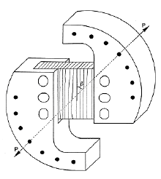
\includegraphics{Figures/Specimen_test}
	\decoRule
	\caption[CTS specimen]{CTS specimen tested in mode III by angular loads}
	\label{fig:CTS}
\end{figure}
One interest of this type of sample is that this test is possible in crack opening mode, but also in shear mode or in mixed mode. Another  advantage is linked to these dimensions, smaller than those of DCB for instance. This is an interesting point for this work to reduce the volume which must be submerged to gain in MC.

%----------------------------------------------------------------------------------------
%	SUBSECTION 3
%----------------------------------------------------------------------------------------
\subsection{ Mixed Mode Crack Growth (MMCG) specimen}

So many geometries can be used to allow experimental studies. This thesis, inspired on previous work use MMCG specimen which derivate from DCB and CTS specimen presented before. The purpose of MMCG specimen, \parencite{Reference6} is to involve a stable propagation of the crack in different mode and in mixed mode too. The study of this sample uses the rate of refund (G). G decrease while the crack is developing, until sample rupture. Tests on MMCG specimen can be study thanks to finite elements like the J integral method, which is used in this work. But also, by image analysis, like the DIC analysis.
\begin{figure}[th]
	\centering
	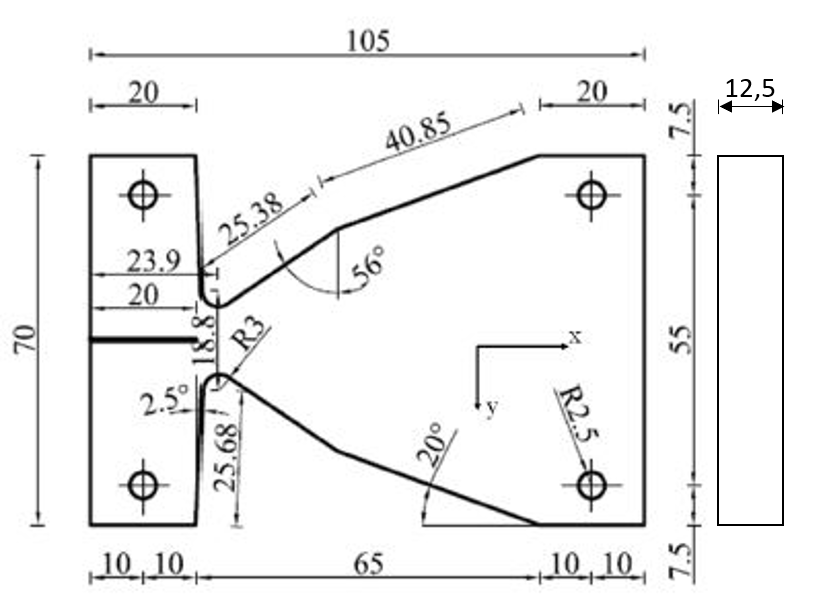
\includegraphics[scale=0.5]{Figures/MMCG_specimen}
	\decoRule
	\caption[MMCG specimen]{dimensions and geometry of Mixed Mode Crack Growth specimen}
	\label{fig:Fig5}
\end{figure}
MMCG sample is a compromise between DCB and CTS samples to obtain different mixing rates and a stable crack propagation. It is the specimen which will be used for this Development and Research Project, because of the good stability of the sample, presented in \parencite{Reference6} thesis. The Geometry, visible on \ref{fig:Fig5} was already tested in \parencite{Reference7} works. Manufactured samples of Okoume species with these dimensions were available in Polytech laboratory.

MMCG shapes are linked to Compact Tension Shear (CTS) specimen due to the tiny dimensions of MMCG samples which are similar to CTS ones. This geometry involves a little Fracture Process Zone (PFZ) which begin at the crack tip. But at the contrary of DCB specimen, the smaller dimensions of MMCG specimen does not allow a long displacement of the PFZ during the test. So after few minutes of displacement of the crack tip, the specimen will break. It is linked to DCB specimen because of \parencite{Reference10} work and the creation of variable inertia in DCB specimens. It must be noted, that the chosen MMCG specimen are RL samples so with a Radial and Longitudinal surface. The Tangential direction corresponds to the thickness of specimens. It means that the  swelling principally involves an expansion of the specimen thickness.

In mode one, a really progressive crack is expected. As it was said, \parencite{Reference6} developed this particular shape, to improve the stable propagation of the crack, more than in a DCB sample. Moreover, the different angles shown on \ref{fig:Fig5} and the rounded chamfer provide uncontrollable collapse of the specimen. Indeed, the optimization consists, on the variable inertia also used in DCB specimens. It was proved by Finite Element Analysis (FEA) that the connection between the heels and the body of the specimen is a zone where strains are concentrated. These shapes, allow by limiting the surface, to avoid wood heterogeneity. Besides, this compact geometry involves a faster increase of the MC in the specimen. It is logical but can be reminded by \ref{eq:moisture flux in wood}

\begin{equation}
\begin{array}{l}
	q_{m}= -\rho_{0}\cdot D \cdot \bigtriangledown m 
	\\
	\\
	\left\{
	\begin{array}{lll}
	q_{m}: & $moisture flux$ & \si{\square\meter\per\second} \\
	D: & $Diffusivity$ & \si{\square\meter\per\second} \\
	\bigtriangledown: & $Gradient$ & . \\ 
	m: & $moisture content$ & \% \\
	\end{array}{}
	\right.
\end{array}{}
	\label{eq:moisture flux in wood}
\end{equation} 


%----------------------------------------------------------------------------------------
%	SUBSECTION 4
%----------------------------------------------------------------------------------------
\subsection{ Climatic effects on the test }

This work studies the impact of temperature and moisture content variation on wood samples. The moisture content have an impact on the studied parameters as the energy rate or the mechanical resistance. Moreover, it is a phenomenon, present in the wild, which participate to wood life. Non precise technics allow to have an idea of the moisture content in the wood. But every specie is different and even, each tree is different. 
Without moisture meter, the moisture content in our specimens is determined by the weight measurement of the sample. The concept is to dry the specimen to obtain the anhydrous weight. Thanks to this measure ($M_{0}$), and the actual weight ($M_{S}$) the \ref{eq:Moisture content depending on weight} is :
\begin{equation}
	H=\frac{_{M_{S}-M_{0}}}{M_{0}}100
	\label{eq:Moisture content depending on weight}
\end{equation} 

The species presented were chosen among many others for different reasons. First, they have an interesting and different behavior. Indeed, they have different density but also mechanical behavior and are from different area and type of woods, as explained before. Then, there are really linked to the Civil engineering subject. Except Okoume specie, all the other are not enough exploited for construction uses. Gabon forest are composed of many wood, but without the use of some of them in construction field, as for Iroko and Padouck species. In France, the same fact appears in Massif Central forest, composed of many Silver Fir areas. By proving that these species have a good behavior in humid environment, it could allow, their use in Construction field. Looking to \parencite{Kif1998}, \parencite{Ang2017}, \parencite{Huang2020} works presenting wood behavior at different moisture content, or \parencite{Seif2017} for severals temperature, some values can be expected. Indeed, it is not the first work on this subject and our results could be discussed according to other articles.

Indeed, researches were also, already done on the subject, like \parencite{Reference12} studied on Jack pine (Pinus banksiana) and balsam poplar. He observes the mechanical properties of wood, function of the moisture content and temperature. It appears that another possibility to modify the moisture content, is the use of solution. \parencite{Reference12} presents three principal solutions, placed in a desiccator: MgCl2, NaNO3 and KCl. 

Another climatic condition, which must be considered, is the temperature. The temperature can involve an augmentation of moisture content. Tests are done on this sample at normal temperature, but also at a lower one by putting specimen during 48 hours into a fridge. This experiment allows to prove the gain of moisture content due to the decreasing temperature. Scientists as \parencite{Reference13} did tests on sample under different temperature, 20\textcelsius, 40\textcelsius, 60\textcelsius and 80\textcelsius but also 100\textcelsius to 200\textcelsius during two hours for some DCB samples.
Tested samples were DCB ones and the species were Spruce and Beech. Results from works as \parencite{Reference12} on Balsam Poplar, but with compressive tests in a radial direction, allow to have an idea of the way to proceed and the attempt results. 

\begin{table}[h]
	\centering
	\begin{tabular}{cccc}
		\hline
		\rowcolor[HTML]{BFBFBF} 
		\multicolumn{1}{c}{\cellcolor[HTML]{BFBFBF}Reference} & \multicolumn{1}{c}{\cellcolor[HTML]{BFBFBF}Specie} & \multicolumn{1}{c}{\cellcolor[HTML]{BFBFBF}Climatic Variation} & \multicolumn{1}{c}{\cellcolor[HTML]{BFBFBF}Result} \\
		\multicolumn{1}{c}{\cellcolor[HTML]{FFE699}\cite{Kif1998}} & \multicolumn{1}{c}{Scots Pine} & \multicolumn{1}{c}{Earlywood Green} & \multicolumn{1}{c}{$\sigma$ = 49MPa} \\
		\multicolumn{1}{c}{\cellcolor[HTML]{FFE699}\cite{Kif1998}} & \multicolumn{1}{c}{Scots Pine} & \multicolumn{1}{c}{Latewood Green} & \multicolumn{1}{c}{$\sigma$ = 74MPa} \\
		\multicolumn{1}{c}{\cellcolor[HTML]{FFE699}\cite{Kif1998}} & \multicolumn{1}{c}{Scots Pine} & \multicolumn{1}{c}{Earlywood resoaked} & \multicolumn{1}{c}{$\sigma$ = 36MPa} \\
		\multicolumn{1}{c}{\cellcolor[HTML]{FFE699}\cite{Kif1998}} & \multicolumn{1}{c}{Scots Pine} & \multicolumn{1}{c}{Latewood resoaked} & \multicolumn{1}{c}{$\sigma$ = 55MPa} \\
		\multicolumn{1}{c}{\cellcolor[HTML]{B4C6E7}\parencite{Ang2017}} & \multicolumn{1}{c}{Douglas Fir} & \multicolumn{1}{c}{9\% MC} & \multicolumn{1}{c}{$G_{max}$= 780J/$m^{2}$} \\
		\multicolumn{1}{c}{\cellcolor[HTML]{B4C6E7}\cite{Ang2017}} & \multicolumn{1}{c}{Douglas Fir} & \multicolumn{1}{c}{18\%MC} & \multicolumn{1}{c}{$G_{max}$= 680J/$m^{2}$} \\
		\multicolumn{1}{c}{\cellcolor[HTML]{B4C6E7}\cite{Ang2017}} & \multicolumn{1}{c}{White Fir} & \multicolumn{1}{c}{9\% MC} & \multicolumn{1}{c}{$G_{max}$= 580J/$m^{2}$} \\
		\multicolumn{1}{c}{\cellcolor[HTML]{B4C6E7}\cite{Ang2017}} & \multicolumn{1}{c}{White Fir} & \multicolumn{1}{c}{18\%MC} & \multicolumn{1}{c}{$G_{max}$= 630J/$m^{2}$} \\
		\multicolumn{1}{c}{\cellcolor[HTML]{C6E0B4}\cite{Huang2020}} & \multicolumn{1}{c}{Jack Pine} & \multicolumn{1}{c}{2\% MC} & \multicolumn{1}{c}{$\sigma$ = 4,5MPa} \\
		\multicolumn{1}{c}{\cellcolor[HTML]{C6E0B4}\cite{Huang2020}} & \multicolumn{1}{c}{Jack Pine} & \multicolumn{1}{c}{17\% MC} & \multicolumn{1}{c}{$\sigma$ = 2,9MPa} \\
		\multicolumn{1}{c}{\cellcolor[HTML]{C6E0B4}\cite{Huang2020}} & \multicolumn{1}{c}{Balsam Poplar} & \multicolumn{1}{c}{2\% MC} & \multicolumn{1}{c}{$\sigma$ = 5,4MPa} \\
		\multicolumn{1}{c}{\cellcolor[HTML]{C6E0B4}\cite{Huang2020}} & \multicolumn{1}{c}{Balsam Poplar} & \multicolumn{1}{c}{17\% MC} & \multicolumn{1}{c}{$\sigma$ = 3,7MPa} \\
		\multicolumn{1}{c}{\cellcolor[HTML]{F4B084}\cite{Seif2017}} & \multicolumn{1}{c}{Numerical} & \multicolumn{1}{c}{-10 °C} & \multicolumn{1}{c}{G = 8J/$m^{2}$} \\
		\multicolumn{1}{c}{\cellcolor[HTML]{F4B084}\cite{Seif2017}} & \multicolumn{1}{c}{Numerical} & \multicolumn{1}{c}{0 °C} & \multicolumn{1}{c}{G = 9J/$m^{2}$} \\
		\multicolumn{1}{c}{\cellcolor[HTML]{F4B084}\cite{Seif2017}} & \multicolumn{1}{c}{Numerical} & \multicolumn{1}{c}{10 °C} & \multicolumn{1}{c}{G = 11J/$m^{2}$} \\
	\end{tabular}
	\caption{Approximative results from previous works on climatic conditions affecting wood behavior.}
	\label{tab:ArticleResult}
\end{table}

The last climatic conditions, presented is the fatigue load. Even if it is not a real climatic effect, it could be involved by the climate like a snow load. This is the last experiment which will be done on the specimen. Fatigue is directed by Paris law, as the \ref{eq:Paris law, fatigue loads equation} :
\begin{equation}
	\frac{\partial a}{\partial N}=C \Delta K^{m}
	\label{eq:Paris law, fatigue loads equation}
\end{equation} 
With “a”, the crack length, “N” the number of loading cycles, which involve that $\frac{\partial a}{\partial N}$ is the crack growth rate. It depends on the cyclic stress intensity factor $\Delta K$. Finally, “C” and “m” are empirical constants depending on the studied material, but also the frequency, the load ratio, the temperature... This equation allows anticipating crack growth rate and predict fatigue comportment of the material.  

So it is expected that with an increase of the moisture content, the mechanical behavior must decrease, while by increasing the temperature of the specimen, the mechanical behavior should increase, as it is visible in \ref{tab:ArticleResult}. However, this fact will also depend on the specie study.
Linked to the Moisture Content, if the temperature increase, there are less MC into the specimen, so it is expected that with a higher temperature, wood behavior should be better.

%----------------------------------------------------------------------------------------
%	SECTION 4
%----------------------------------------------------------------------------------------
\section{Wood fracture mechanics}


%----------------------------------------------------------------------------------------
%	SUBSECTION 1
%----------------------------------------------------------------------------------------
\subsection{Fracture modes and process zones}

Fracture mechanic has an objective to characterize the cracking behavior of structures through stress field, crack size and cracking resistance of the material.

There are different rupture modes involve by the crack, the direction of the force which create the crack or compounds it. The first mode, called opening mode, characterized by a force applied, perpendicularly to the crack. The shearing mode is the second mode. The force is applied parallelly to the crack. And the third mode of rupture parallelly to the interior of the crack. The principals rupture mode are the first and the second, and this literature review will focus on first mode particularly. These modes are presented on \ref{fig:Fig3}. This first mode can be presenting by the energy release rate (G) linked to time or in our case, crack length, this plot is called R-curve.
\begin{figure}[th]
	\centering
	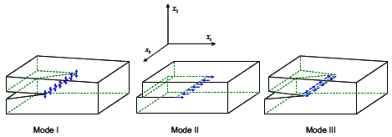
\includegraphics{Figures/Mode_presentation}
	\decoRule
	\caption[Crack modes]{Crack modes depending on the direction of the applied force.}
	\label{fig:Fig3}
\end{figure}
Four zones characterized this propagation crack. The first is a stationary phase, with an increase of G until a critical value in mode 1, “$G_{IC}$” reached at a critical time, called tc. Then a second phase correspond to the crack propagation and occurs at a constant value of G. In the third zone, G decrease and the crack propagation stop. At least, the fourth phase involve material ruin shown by G fast increase, which correspond to an instability.

There are different types of cracks. The crack depends on the microscopic structure of the material, the loading conditions, and many other factors.

Rupture by brutal cracking : it happens on materials with a very high resistance, the working stresses are very high. The presence of small cracks can cause this sudden rupture without plastic deformation. 
Rupture by successive growth of cracks : Also called fatigue failure. The mechanical factors that influence this phenomenon is displacements, strains, and stresses, but also environmental conditions such as temperature or relative humidity. It is easier to observe because it takes more time to involve samples destruction than a unique and sudden crack. Indeed, it is a succession of small cracks from an initial crack. In experimental works, it is often created by a circular saw and the last millimeters of the initial crack, are made by a cutter.  

The test done is filmed to determinate how the cracks will be developed over time, depending on the applied forces. With a material like wood, successive cracks rupture are expected. It is important to notice that different zones are studied. There are three areas. 

First one is the development zone: It is the closest zone to the crack. The study is difficult due to the high stresses which cause irreversible damage to the material. The stress field into the crack is maximal. Indeed, the constraints are modelled, as explained with the equation \ref{eq:stress term σ_11} :
\begin{equation}
	\left\{
	\begin{array}{rcr}
		\sigma_{11}=\frac{K_{1}}{(\sqrt{2 \pi r})}Re[\frac{s_{1}s_{2}}{(s_{1}-s_{2})}(\frac{s_{2}^{2}}{\sqrt{\rho_{2}}}-\frac{s_{1}}{\sqrt{\rho_{2}}})]+\frac{K_{2}}{(\sqrt{2 \pi r})}Re[\frac{1}{(s_{1}-s_{2})}(\frac{s_{2}^{2}}{\sqrt{\rho_{2}}}-\frac{s_{1}}{\sqrt{\rho_{1}}})]	
	\end{array}
	\right.
	\label{eq:stress term σ_11}
\end{equation} 

So, if the study is close to the bottom crack, the “r” factor will decrease, and the constraints will approach to infinite values.

\begin{figure}[th]
	\centering
	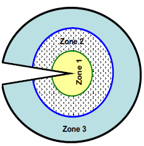
\includegraphics{Figures/Crack_zones}
	\decoRule
	\caption[Crack zones]{Names of each part of the crack}
	\label{fig:Fig4}
\end{figure}

The second zone, visible on \ref{fig:Fig4} is called singular zone: it circled the first zone. The mechanical field does not depend on specimen geometry. Interface between zone one and two, has continuous constraints and displacements values.

The last zone is the farthest zone from the crack tip. It is the zone which is in contact with loads and displacements forces.

%----------------------------------------------------------------------------------------
%	SUBSECTION 2
%----------------------------------------------------------------------------------------
\subsection{Mechanical fields}
There are 2 mechanical fields, isotropic and orthotropic fields. Because of wood behavior, the orthotropic mechanical filed will be the only one presented. 
The elastic stress field, near the crack tip, depends on the material. For an orthotropic material, the expression, presented in \parencite{Reference10} work are :

\begin{equation}
	\left\{
	\begin{array}{rcr}
		\sigma_{11}=\frac{K_{1}}{(\sqrt{2 \pi r})}Re[\frac{s_{1}s_{2}}{(s_{1}-s_{2})}(\frac{s_{2}}{\sqrt{\rho_{2}}}-\frac{s_{1}}{\sqrt{\rho_{2}}})]+\frac{K_{2}}{(\sqrt{2 \pi r})}Re[\frac{1}{(s_{1}-s_{2})}(\frac{s_{2}^{2}}{\sqrt{\rho_{2}}}-\frac{s_{1}^{2}}{\sqrt{\rho_{1}}})]\\
		\sigma_{22}=\frac{K_{1}}{(\sqrt{2 \pi r})}Re[\frac{1}{s_{1}-s_{2}}(\frac{s_{1}}{\sqrt{\rho_{2}}}-\frac{s_{2}}{\sqrt{\rho_{1}}})]+\frac{K_{2}}{(\sqrt{2 \pi r})}Re[\frac{1}{(s_{1}-s_{2})}(\frac{1}{\sqrt{\rho_{2}}}-\frac{s_{1}}{\sqrt{\rho_{1}}})]\\
		\sigma_{21}=\sigma_{12}=\frac{K_{1}}{(\sqrt{2 \pi r})}Re[\frac{s_{1}s_{2}}{(s_{1}-s_{2}}(\frac{s_{1}}{\sqrt{\rho_{1}}}-\frac{1}{\sqrt{\rho_{2}}})]+\frac{K_{2}}{(\sqrt{ 2\pi r})}Re[\frac{1}{(s_{1}-s_{2})}(\frac{s_{1}}{\sqrt{\rho_{2}}}-\frac{s_{2}}{\sqrt{\rho_{1}}})] \\
	\end{array}
	\right.			
	\label{eq:stresses terms from Orthotropic field}
\end{equation} 

In these equations presented in \ref{eq:stresses terms from Orthotropic field}, $S_{i}$ with i = {1;2} are the polynomial roots calculated by another equation, using the components of the stiffness tensor for an orthotropic symmetry. 
Therefore, terms
\begin{equation}	
	\rho_{j}=\cos{\theta}+i s_{j} \sin{\theta} and j\in{[1;2]}
	\label{eq:terms present in stress equations}
\end{equation}			
These theories, are already used, and the orthotropic equations will be those that will be used for wood experiments. Indeed, even if the resolution could be done by ourselves, there are nowadays, computer software, which allow us to spend less time resolving orthotropic equations. It is written in the software program, and run, until finding solutions.

%----------------------------------------------------------------------------------------
%	SUBSECTION 3
%----------------------------------------------------------------------------------------
\subsection{Stress Intensity Factor}
K is  the stress intensity factor, and $K_{Ic}$, is the one for the opening mode. The "c" means that it is the critical value of this coefficient. As \parencite{Reference10} explains, by using Laplace Carson inverse on Stress Intensity Factor (SIF), it is possible to obtain crack opening factors. Focusing on mode I, it is particularly interesting to understand how $K_{Ic}$ evolves. The stress intensity factor K can be obtained by using finite element analysis (for example, with a contour integral method for orthotropic materials). It is obtained with the initial crack length $a_{initial}$ linked to the crack length L : $\frac{a_{initial}}{L}$.
The stress intensity factor depends on the specimen geometry. The classic linear elastic fracture mechanics equation for SIF is presented in \ref{eq:Intensity factor}:
\begin{equation}
	K_{I}=\frac{P}{W\sqrt{L}}f\frac{a_{initial}}{L} 	
	\label{eq:Intensity factor}
\end{equation} 						
P : the force applied on the specimen 
W the thickness
L the crack length 
f the linear function which link the terms $a_{initial}$ and L in $\frac{a_{initial}}{L}$. 

It also associated to the Stress Intensity Factor (SIF) name. 

%----------------------------------------------------------------------------------------
%	SUBSECTION 4
%----------------------------------------------------------------------------------------

\section{Energetic methods}

Different methods were created to work on fracture mechanics, called energetic methods. $G_{\theta}$ or $M_{\theta}$ which are defined on surface contours. J and $G_{\theta}$ are useful for pure shearing or opening tests, due to a global energetic operation. All the presented integral with a $\theta$ terms have an important difference. They are defined on a surface contour, which is easier to integrate. M-integral has two terms, depending on real or virtual displacements involving real and virtual constraints, which allow decoupling modes
A-integral is an independent integral which allows to consider the effect of thermo-hygro-mechanical loads in the cracking process. During the crack process, it uses temperatures data. As T-integral, it is similar to M-integral, and do not include the crack tip, which is a particular part of the crack (too many singularities).

In this work, the chosen method, which is created in a Python program to carry out this work is the Rice Integral.

Rice Integral is presented as the next formula \ref{eq:J, Rice integral} :
\begin{equation}
	J=\int_{\Gamma}[F n_{1}-\sigma_{ij} n_{j} \frac{\delta u_{i}}{\delta x_{1}}]d\Gamma
	\label{eq:J, Rice integral}
\end{equation}  

The considered contour of this integral is curvilinear and is named $\Gamma$. It includes the crack tip while it is not the case of others energetic method. “F” is the force applied on each part of the crack tip. Then, “a” is still the length of the crack. “$n_i$“ are the normal vectors to the curvilinear contour $\Gamma_{i}$, and $\sigma$ is the strain used to obtain crack opening. 
There are better energetics methods. As $G_{\theta}$ or $M_{\theta}$ which are defined on surface contours. J and $G_{\theta}$ are useful for pure shearing opening, due to a global energetic operation. But J integral also allows to work on mode I cases. Then we will also use the compliance method to obtain the energy release rate.

%----------------------------------------------------------------------------------------
%	SUBSECTION 4
%----------------------------------------------------------------------------------------

\section{Compliance method}

Compliance is the characterizing quantity of material elasticity behavior. An elasticity compliance corresponds to the inverse of material elastic modulus. Its unity is the $Pa^-1$.
Compliance method is used to determinate the crack resistance. 
The formula used to calculate this energy release rate is written on \ref{eq:Energy release rate equation}:
\begin{equation}
	G_{c}= \frac{F_{c}^2}{2b} (\frac{\Delta C}{\Delta a})_{d} 	
	\label{eq:Energy release rate equation}
\end{equation}  
With : 
$G_c$ the value of energy release rate (in \si{\joule\per\square\meter})
$F_c$ the critical force which involves the crack (in \si{\newton})
b the thickness of the specimen (in \si{\milli\meter})
$\Delta C$ the compliance evolution (in $Pa^-1$)
$\Delta a$ the crack length evolution (in \si{\milli\meter})
In this work, C is determined in forced displacement, by the division of U, which is the imposed displacement, by F, the applied force. It must be noted that to have an idea of the imposed displacement depending on time, some articles as \parencite{Reference7} or \parencite{reference15} allow to fix this displacement between 2\si{\milli\meter\per\minute} until 5\si{\milli\meter\per\minute}.

As explained in previous part, the specimen presenting a RL surface studied have a Tangential dimension for their thickness. It involves a dimension evolution of this parameter. So for each test at a different MC, the b parameter must be measured, in order to have a precise value of G. Compliance method is often used in mode I analysis. It was the way of study for works as \parencite{Reference7}, \parencite{Ang2017}...

%----------------------------------------------------------------------------------------
%	SECTION 5
%----------------------------------------------------------------------------------------
\section{Software programms and analyzing tools}

%----------------------------------------------------------------------------------------
%	SUBSECTION 1
%----------------------------------------------------------------------------------------
\subsection{Image Correlation knowledges}

Image analysis is a powerful tool. Indeed, the number of domains using it is numerous. Everybody has already seen the facial recognition system working. It is similar to the fracture mechanic uses. It works by comparing two images, a first one putted in the system, and another when a person wants to unlock the system. If the two images are similar with a percentage of error, it will work.
The first use was for fluid mechanic. It was the first field which used image analysis. Indeed, it was easier with old camera to follow a moving point into fluid, than a point into a solid, because the displacement is smaller and difficult to observe if the resolution is not good enough.
Agronomic field is concerned too. Fernando Mendoza work explain how image analysis is used to determinate apples properties. Indeed, by analyzing apple images, he can determinate the optimal day for the harvest. He looks at special characteristics, like firmness and soluble solids content to obtain the best apple for consumers.

To focus on the one used in this work, digital measurement techniques using pictures, is a really interesting tool to work on fracture mechanics. Digital Image Correlation (DIC) consists in comparing two images of the same object on load, as MMCG specimen in our case, and looking to the displacement field, in order to find a match between the two images. When a series of images is obtained, the comparison between these images, and their differences are analyzed very accurately, pixel by pixel to obtain the real displacements, from one point to another place. The main problem of this technique is due to “noise” which involve uncertainties. Therefore, light problems can occur and decrease the precision of the results. In this method it is necessary to extract the two images (before and after movement).

The DIC method is based on the principles of mechanical continuity (rigid body mechanics). The system consists of using a digital camera and specialized computer software, in this work, MatchID. Camera is used to capture consecutive images of the tested sample surface during the deformation test. Digital images determined by this way, which corresponds to a series of photos, is analyzed by the DIC software. Displacement maps of specimen on the surface is created. Stress fields can be evaluated from strain fields. The formula used to obtain the displacement field is shown in \ref{eq:displacement field obtained by DIC methods}

\begin{equation}
	u^{k}=
	\begin{bmatrix}
		u_{z}^{k}\\u_{y}^{k}
	\end{bmatrix}
	=\Sigma^{N}_{i=1}
	\begin{bmatrix}
		f_{i}(k,\phi_{k}) & g_{i}(k,\phi_{k})\\ l_{i}(k,\phi_{k}) & m_{i}(k,\phi_{k})
	\end{bmatrix}
	\begin{bmatrix}
		A^{i}_{1}\\A^{i}_{2}
	\end{bmatrix}
	\begin{bmatrix}
		r^{i/2}_{k}
	\end{bmatrix}
	+
	\begin{bmatrix}
		T_{x}\\T_{y}
	\end{bmatrix}
	+
	R
	\begin{bmatrix}
		y_{k}\\y_{k}
	\end{bmatrix}
	\label{eq:displacement field obtained by DIC methods}
\end{equation} 

With $f_{i}$, $g_{i}$, $l_{i}$, $m_{i}$, polar functions, k is depending on the material because of Poisson term which determinates k. T terms are correction factors for rigid body motions.
Due to the fast and easy preparation, it is a very used fracture mechanic technique. After the determination of the displacement field, by using the integral method presented in last sections, it is possible to obtain the strain field.

If this method is used on wood, it is important to note that elastic orthotropic material model in 2D has five engineering constants as input parameters, to enter in the image analysis system. Even if it depends on the software used, these inputs are important to be known. First, Young modulus in longitudinal direction must be informed, $E_{L}$=$E_{1}$, transverse Young modulus $E_{trans}=E_{R}=E_{T}=E_{2}$. Then, shear modulus $G_{LR}=G_{LT}=G_{12}$, if shearing mode is studied. Therefore, Poisson coefficient $\nu$ has to be put into the software. This coefficient can change depending on the studied surface, in or out the plan. The initial crack length is introduced in the model. The damage description is presented by three principal inputs, even if it could change, depending on the software. Focusing on mode I damage, it is described by damage initiation stress $\sigma_{ini}$, but also separation at the failure $\delta_{fl}$, and exponential function shape coefficient $\alpha_{I}$. 

Beside, other technics could allow to do the same analysis. The only changement is linked to the pattern put on the specimen to follow the displacement and deduct the strain field. It could be a grid as in \parencite{Reference7} work or a marker.

%----------------------------------------------------------------------------------------
%	SUBSECTION 2
%----------------------------------------------------------------------------------------
\subsection{Analysis Software}

One of this work purpose, was to compare experimental wood behavior and analytic one.
Numerical simulation is a representation of complex physical phenomena. This is a way to virtually simulate a product in its final environment or submitted to different stress. In this work case, the fracture propagation was the physical phenomenon which have to be simulated. To do this job, many software tools were available. SolidWorks was a great candidate. Indeed, it is easy to use it and find tutorial to quickly learn. A try was done as visible on \ref{fig:SolidWorks}. As presented in \parencite{Reference8} and visible on \ref{fig:SolidWorks} thesis three areas are more impacted than the others. It must be noted, that before creating Okoume material on SolidWorks, steel was applied on this MMCG shape, in order to have a look on the behavior. By imposing 20\si{\milli\meter} of displacement, the specimen collapse, occurs in the holes' area. In the current example, a force is applied on the heel to avoid the bending moment which occurs on the upper heel. Indeed, by the application of the load in the upper hole, this part of the specimen is bending. The heel load is like a boundary condition as the one applied in the other hole. The \ref{fig:SolidWorks} example is an Okoume specimen with a 1\si{\centi\meter} notch. A static test is done by the traction from one hole at a load of 400\si{\newton}. This load is higher than the values given by \parencite{Reference7} thesis but allow to obtain values. So even if SolidWork is not as complete as others, this software permit the highlight of constraints areas. Indeed it is not possible to follow a crack evolution or really use the temperature or humidity coefficient to impact an experiment.

So the chosen software was Abaqus.
Indeed, to proceed a non-linear and multi-physics experiment, as with an orthotropic material submitted to climatic condition changes, Abaqus seems to be the best software. It allows to work on complex materials. Indeed, Abaqus makes possible to set up very complex and personalized material behaviors, including the definition of failure criteria. The user can use metallic, hyper-elastic, plastic or even composite materials. In addition, the material properties can also vary depending on field variables such as temperature.

Abaqus, also allows working on non linearity problem. Indeed, the contact resolution algorithm is very powerful. It takes into account very complex contact behaviors which consider large rotations and friction.  It is possible to work on static and dynamic problems, in 2D or 3D.
On this software, it is possible to create shape of the part on other application as CATIA or SolidWorks. Indeed, associative interfaces allow the transfer of geometry from a CAD system to Abaqus.

It works as a Finite Element Method solver. The procedure is user-friendly. First, it is necessary to create the shapes of the specimen which will be tested experimentally, in this case a MMCG specimen. This creation system is not as intuitive as the others steps. But by importing the shapes from another software, it can make the task easier. Then the different stages are presented by the interface as on \ref{fig:Abaqus_interface}.
\begin{figure}[th]
\centering
\begin{subfigure}{0.48\linewidth}
\centering
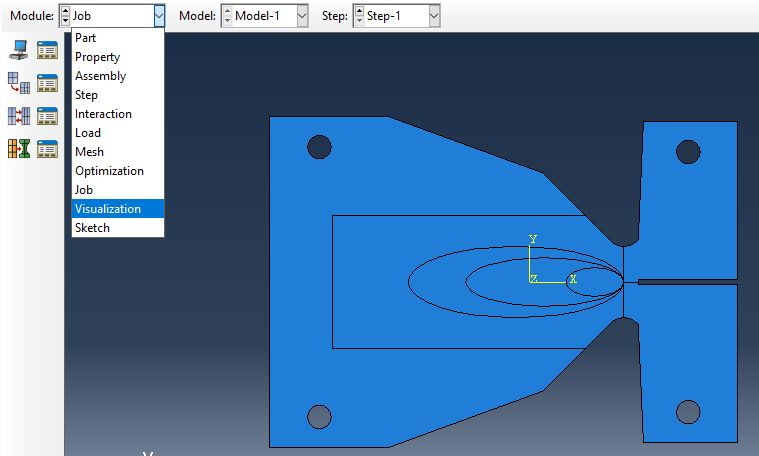
\includegraphics[scale=0.5]{Figures/Abaqus_fct}
\decoRule
\caption[Abaqus interface]{Different stages for Abaqus creation model presented next to a MMCG specimen part}
\label{fig:Abaqus_interface}
\end{subfigure}
\\
\begin{subfigure}{0.48\linewidth}
\centering
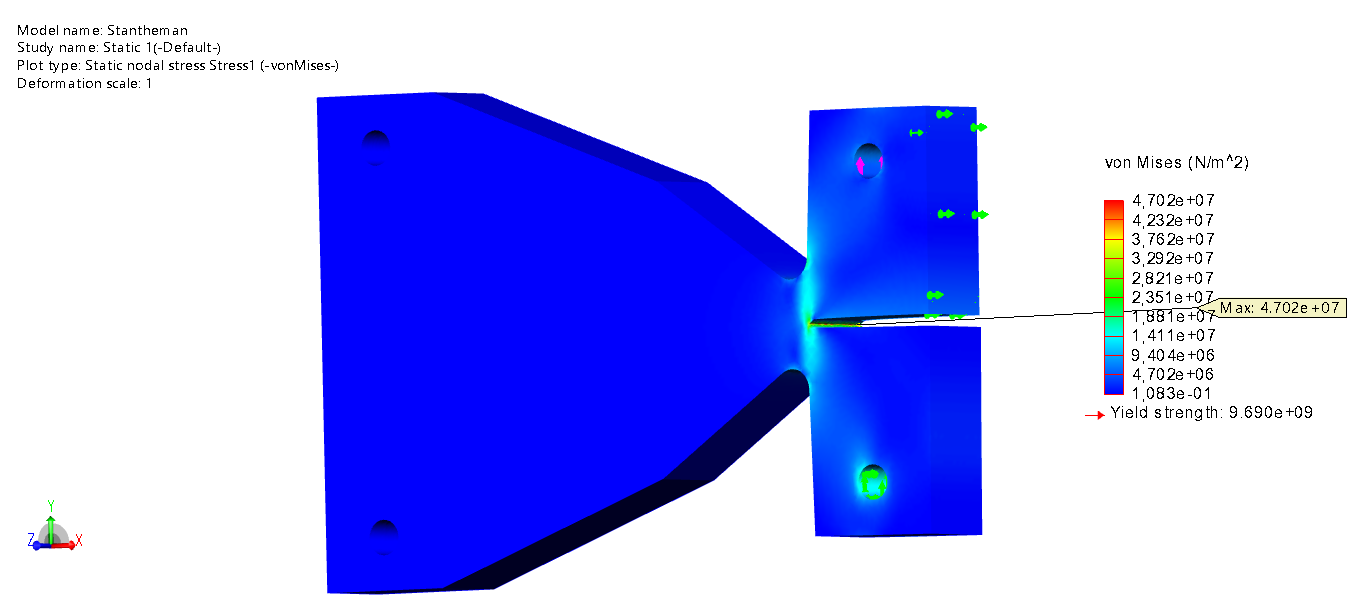
\includegraphics[scale=0.35]{Figures/SolidWorks}
\decoRule
\caption[SolidWorks analysis of Okoume specimen]{Example of SolidWorks analysis on Okoume specimen loaded }
\label{fig:SolidWorks}
\end{subfigure}
\caption[Software analysis]{Software analysis}
\label{fig:Softwares}
\end{figure}
So after creating the shapes, a material must be added to the part. By creating an entire material, the true values of Okoume, PAdouck and Iroko can be associated to the shapes. Then, some interaction must be input, as the force applied on the part or the boundariy condition. An automatic mesh can be created. But with a student license only 1000 nodes can be created. So the mesh is not as precise as it could be, due to the important dimensions of the mesh element. One solution is to refine some of the studied areas and let other surface with bigger mesh elements. Looking to steps created before, it is possible to do a crack modulus job to observe the crack propagation on the drawn specimen. The job allow to follow the crack and have a look to the strain map or the displacement one. Each element of the mesh will give information about the evolution of the crack in this work case. This crack modulus analysis is not available on SolidWOrks. 

%----------------------------------------------------------------------------------------
%	SUBSECTION 3
%----------------------------------------------------------------------------------------
\subsection{Programmation tools}

Even if DIC is really powerful, the treatment of the data, needs other tools. Programmation is an interesting way to proceed. 
First, a solution was to put all the values as CSV file into an Excel table and use VBA programmation to proceed. But the number of stage and the number on data is too important. So real programmation tool were needed.

Previous work as \parencite{Reference14} ones were done on MatLab. It is a software program for performing numerical calculations. It was originally designed to facilitate the processing of matrices. So a really interesting tool in work using big matrix as this one. But it is now used in all areas of sciences that require calculations more than just matrix operations. There are many interests as :
\newline
the fact that it is a faster programming for calculation and plotting curve. There are possibilities of including programs from other programmation language as C or C ++. It is a self interpreted language, so no compilations are needed which provide compiling wait. And it is also easy to understand the code which is a very readable one. In another hand, some disadvantages can be found, like :
\newline
The calculation speed is slower than in C or C ++ languages. This software tool must also be paid. Indeed, even for students, an activation key has to be given by the school, while other language, like Scilab, are totally free and equivalent.

Matlab is used to do computational experiments very quickly. Some programs that would require one day of programming in C ++ can be done in 1 hour with Matlab. But when everything is programmed, the computation time in Matlab can be 100 times greater than  C ++ one. For this reason and to use a free software program usable by all, Python was chosen.

Indeed, Python has also many advantages. Like MatLab, it is possible to write part of your code in other programmation languages like C languages. But the reverse is also possible, for instance, if the Python code from this work must be added in another type of software program.
Python is also extremely used and becomes universal, it constitutes other languages or software program like Raspberry Pi. And it also can be used directly in these software programs, as it is the case in Abaqus or Ansys. Like MAtLab, it is a readable and user-friendly language. It is also possible to use certain codes previously created in the one which is in creation. For this reason, persons wanting to work on a subject linked to the one presented here, will be able to reuse the code and call it, even if it is only for the determination of a single parameter as the crack length or the crack tip opening displacement. Most importantly, it has a very large package library that allows to quickly add improvements to existing code. When it is downloaded, Python includes a complete library containing code allowing for example the use of expressions or the generation of documentation, databases, image manipulation. But one of the most used Python tool in this work is the VCS option, which create a "shared" Python code. Indeed with the GitHub online software tool, it was possible to share an entire folder containing Python code, but also the report below in Latex, the Excel documents, the modeling files under Abaqus ... Thanks to this tool, all these files were accessible and readable by all, allowing real-time monitoring of each work tool. In addition, after each update, by one of the members having access to the file, the changes are presented separately. Finally, a new option on Python allows to work on the same program at the same time as a Google Doc text document would allow. However, it is important to have some basic knowledges in programmation. Indeed, even with some courses on VBA and C language, it takes time to take charge of this tool. But again, it is a really used language, and many forums allow to find solutions.

%%%%%%%%%%%%%%%%%%%%%%%%%%%%%%%%%%%%%%%%%%%%
%%%%%%%%%%%%%%%%%%%%%%%%%%%%%%%%%%%%%%%%%%%%


%
%\subsection{Softwares and Match ID utilisations}
%
%First it was decided to present one software for each method. Regarding the methods operation, it appears that they work with similar softwares. Indeed, as presented in last section, the method is always the analysis of two images and determining which are the differences. The only changes is the pattern on the sample, a grid, a marker, or the initial surface if it is not too uniform.
%Aramis system develop software but also equipment to allow the best capture and resolution of images. It is used for DIC. 
%Match ID will be the used software. 
%
%\begin{figure}[th]
%	\centering
%	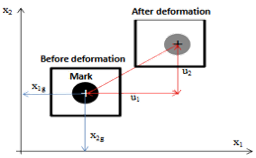
\includegraphics{Figures/Subset_Movement}
%	\decoRule
%	\caption[Subset Displacement]{Tracking markers scheme with the displacement of a mark before and after a deformation}
%	\label{fig:Fig7}
%\end{figure}
%
%The MatchID software was chosen to compute DIC images and obtain displacement field and strain one. It is a powerful software with a new option which is linked to “crack” studies.
%Thanks to this software, some ”.csv” files full of information were available. All the images recorded were treated with MatchID and every picture are divided into a large number of subsets. One subset is composed of 225pixels (square of 15 by 15 pixels). It is possible to have a look on the crack video, watch the different strains modelized by MatchID using every pixel’s evolution. Then the user must determine the initial length. Indeed, even if the specimens were manufactured with a precise shape, it was important to calibrate the initial length of the crack, by choosing the subset the closest to the crack tip.
%When all these steps are done, for each experiment, so each specimen, a database have to be created. In these databases, will be found constant and information as this initial crack length $a_{0}$. Moreover, there is information, common to each test as the specimen geometry, filmed values or conversion factors.
%
%As it is visible on \ref{fig:Fig7} DIC process works as Finit Element Method (FEM). Indeed a subset can be considered as an element of the project and then, looking to his displacement, strains and displacement map can be plot. The next section, will allow to better understand how a comparison between FEM and experiment can be done.
%
%
